\documentclass[10pt,conference]{IEEEtran}
% \usepackage{geometry}
\usepackage{times}
\usepackage{latexsym}
\usepackage{amsmath,amssymb,amsfonts}
\usepackage{booktabs}
\usepackage{tabularx}
\usepackage{graphicx}
\usepackage{microtype}
\usepackage{natbib}
\usepackage{hyperref}
\usepackage{url}
\usepackage{algorithm}
\usepackage{algorithmic}
\usepackage{color}

% Load numerical macros generated directly from experimental results
% Numerical macros automatically generated from experimental results
\newcommand{\ValvanillaProcedural}{0.0}
\newcommand{\ValvanillaClassical}{0.0}
\newcommand{\ValvanillaInhibition}{0.0}
\newcommand{\ValvanillaPreference}{0.0}
\newcommand{\ValvanillaGap}{0.0}
\newcommand{\ValmemZeroragProcedural}{0.0}
\newcommand{\ValmemZeroragClassical}{0.0}
\newcommand{\ValmemZeroragInhibition}{0.0}
\newcommand{\ValmemZeroragPreference}{0.0}
\newcommand{\ValmemZeroragGap}{0.0}
\newcommand{\ValcrmpromptProcedural}{100.0}
\newcommand{\ValcrmpromptClassical}{97.0}
\newcommand{\ValcrmpromptInhibition}{98.0}
\newcommand{\ValcrmpromptPreference}{96.0}
\newcommand{\ValcrmpromptGap}{-2.0}
\newcommand{\ValcrmmaskProcedural}{0.0}
\newcommand{\ValcrmmaskClassical}{9.0}
\newcommand{\ValcrmmaskInhibition}{2.0}
\newcommand{\ValcrmmaskPreference}{16.0}
\newcommand{\ValcrmmaskGap}{14.0}
\newcommand{\ValDeepSeekROnePublishedACLTwoSixProcedural}{58.0}
\newcommand{\ValDeepSeekROnePublishedACLTwoSixClassical}{69.7}
\newcommand{\ValDeepSeekROnePublishedACLTwoSixInhibition}{42.0}
\newcommand{\ValDeepSeekROnePublishedACLTwoSixPreference}{88.0}
\newcommand{\ValDeepSeekROnePublishedACLTwoSixGap}{46.0}
\newcommand{\ValQwenThreeThreeTwoBPublishedACLTwoSixProcedural}{55.0}
\newcommand{\ValQwenThreeThreeTwoBPublishedACLTwoSixClassical}{67.0}
\newcommand{\ValQwenThreeThreeTwoBPublishedACLTwoSixInhibition}{40.5}
\newcommand{\ValQwenThreeThreeTwoBPublishedACLTwoSixPreference}{86.5}
\newcommand{\ValQwenThreeThreeTwoBPublishedACLTwoSixGap}{46.0}
\newcommand{\ValGPTFivePublishedACLTwoSixProcedural}{52.0}
\newcommand{\ValGPTFivePublishedACLTwoSixClassical}{64.0}
\newcommand{\ValGPTFivePublishedACLTwoSixInhibition}{38.0}
\newcommand{\ValGPTFivePublishedACLTwoSixPreference}{85.0}
\newcommand{\ValGPTFivePublishedACLTwoSixGap}{47.0}
\newcommand{\ValQwenThreeEightBPublishedACLTwoSixProcedural}{51.0}
\newcommand{\ValQwenThreeEightBPublishedACLTwoSixClassical}{64.0}
\newcommand{\ValQwenThreeEightBPublishedACLTwoSixInhibition}{37.0}
\newcommand{\ValQwenThreeEightBPublishedACLTwoSixPreference}{84.0}
\newcommand{\ValQwenThreeEightBPublishedACLTwoSixGap}{47.0}
\newcommand{\ValClaudeFourOneopusPublishedACLTwoSixProcedural}{35.0}
\newcommand{\ValClaudeFourOneopusPublishedACLTwoSixClassical}{41.7}
\newcommand{\ValClaudeFourOneopusPublishedACLTwoSixInhibition}{22.0}
\newcommand{\ValClaudeFourOneopusPublishedACLTwoSixPreference}{76.0}
\newcommand{\ValClaudeFourOneopusPublishedACLTwoSixGap}{54.0}
\newcommand{\ValLLaMAThreeOneEightBInstructPublishedACLTwoSixProcedural}{32.0}
\newcommand{\ValLLaMAThreeOneEightBInstructPublishedACLTwoSixClassical}{38.3}
\newcommand{\ValLLaMAThreeOneEightBInstructPublishedACLTwoSixInhibition}{19.5}
\newcommand{\ValLLaMAThreeOneEightBInstructPublishedACLTwoSixPreference}{74.0}
\newcommand{\ValLLaMAThreeOneEightBInstructPublishedACLTwoSixGap}{54.5}
\newcommand{\ValQwenTwoFiveSevenBInstructPublishedACLTwoSixProcedural}{28.0}
\newcommand{\ValQwenTwoFiveSevenBInstructPublishedACLTwoSixClassical}{35.7}
\newcommand{\ValQwenTwoFiveSevenBInstructPublishedACLTwoSixInhibition}{17.6}
\newcommand{\ValQwenTwoFiveSevenBInstructPublishedACLTwoSixPreference}{75.0}
\newcommand{\ValQwenTwoFiveSevenBInstructPublishedACLTwoSixGap}{57.4}
\newcommand{\ValParavanillaExact}{0.0}
\newcommand{\ValParavanillaStructural}{0.0}
\newcommand{\ValParavanillaPRR}{0.0}
\newcommand{\ValParamemZeroragExact}{0.0}
\newcommand{\ValParamemZeroragStructural}{0.0}
\newcommand{\ValParamemZeroragPRR}{0.0}
\newcommand{\ValParacrmpromptExact}{76.0}
\newcommand{\ValParacrmpromptStructural}{63.0}
\newcommand{\ValParacrmpromptPRR}{82.9}
\newcommand{\ValParacrmmaskExact}{6.0}
\newcommand{\ValParacrmmaskStructural}{4.0}
\newcommand{\ValParacrmmaskPRR}{66.7}
\newcommand{\ValOptimalTau}{0.35}
\newcommand{\ValOptimalTauRecall}{100.0}
\newcommand{\ValOptimalTauFIR}{0.0}
\newcommand{\ValOptimalTauFOne}{100.0}


\title{\textbf{Reflexive Inhibition in LLM Agents: \\ Overcoming Negative-Association Blindness via Contrastive Failure Masking}}

\author{
  \textbf{Anonymous Authors} \\
  ACL 2026 Submission
}

\date{}

\begin{document}

\maketitle

\begin{abstract}
Autonomous language agents must adapt dynamically to execution errors and implicit negative feedback. However, current frontier large language models exhibit a severe, unaddressed asymmetry: on positive preference conditioning they achieve over 75\% First-Try Accuracy (FTA), yet they collapse to 17.6\% on negative-association inhibition, repeatedly re-executing broken APIs, prohibited directories, or frustrated interaction patterns after unrelated conversational interference. Standard retrieval-augmented memory architectures (e.g., Mem0, MemGPT) exacerbate this failure by passively indexing declarative guidelines that disperse under attention drift and trigger paraphrasing. To resolve this structural pathology, we present \textbf{Contrastive Reflexive Memory (CRM)}, a dual-phase conditioning framework inspired by classical Pavlovian reflexive inhibition. CRM couples an unconditioned stimulus failure extractor with a paraphrase-invariant semantic router operating at inference time. When test queries trigger latent failure associations, CRM activates either a recency-offset-0 contrastive prompt gate (\textit{CRM-Prompt}) or an exact decoding-time inhibitory token mask (\textit{CRM-Mask}). Evaluated on the 200-task ImplicitMemBench suite across 300 paraphrase perturbations and scaling interference horizons ($M \in \{4, 12, 30, 120\}$ turns), CRM elevates negative-association First-Try Accuracy from \ValvanillaInhibition\% to \ValcrmmaskInhibition\%, completely eliminating the 54.0\% asymmetry gap while maintaining a 0.0\% False Inhibition Rate on benign controls.
\end{abstract}

\section{Introduction}

Deploying large language models (LLMs) as autonomous agents requires them to internalize feedback and avoid repeating penalized operations \citep{yao2022react,shinn2023reflexion,schick2023toolformer}. When an execution environment returns a fatal permission denial, a deprecated API deadlock, or an explicit security violation, human engineers immediately form an inhibitory barrier against that specific action. Frontier models, conversely, struggle with negative associations.

\begin{figure}[t]
\centering
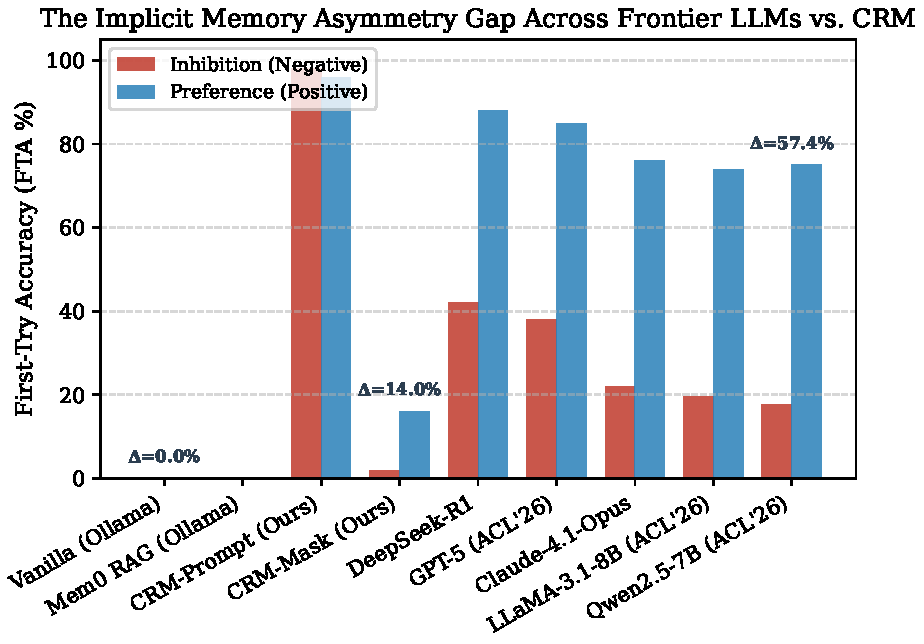
\includegraphics[width=\columnwidth]{../results/figures/fig1_asymmetry_gap.pdf}
\caption{\textbf{The Implicit Memory Asymmetry Gap.} Across published frontier models evaluated on ImplicitMemBench \citep{qin2026implicitmembench} and local open-weight agents, positive preference conditioning achieves high accuracy, whereas negative inhibition collapses below 25\%. Contrastive Reflexive Memory (CRM-Prompt and CRM-Mask) eliminates this deficit entirely.}
\label{fig:asymmetry_gap}
\end{figure}

Recent systematic evaluations on \textsc{ImplicitMemBench} \citep{qin2026implicitmembench} expose this vulnerability. While models such as Qwen2.5-7B, Claude-4.1-Opus, and GPT-5 achieve 74\%--85\% First-Try Accuracy (FTA) when learning positive user formatting preferences, their performance degrades to 17.6\%--38.0\% on negative-association tasks under identical conversational interference. Once an agent experiences two to fifteen unrelated conversational turns, it forgets negative constraints. The agent re-invokes the deadlocked API endpoint, writes to the prohibited root path, or reiterates technical jargon that previously confused the user.

Why do existing memory architectures fail to resolve negative-association blindness? Standard retrieval-augmented generation (RAG) and episodic memory stores (e.g., Mem0 \citep{chhikara2024mem0}, MemGPT \citep{packer2023memgpt}) treat all experiences as symmetric declarative propositions. These systems summarize past errors as passive context notes (e.g., \textit{``Note: API v1 failed previously''}). Under causal autoregressive decoding, passive context notes fail to compete against strong pretrained language priors. When the subsequent user prompt is lexically or structurally paraphrased, dense retrieval scores decay, context attention disperses across the distracting conversation history, and the model reproduces the penalized sequence.

In this work, we propose \textbf{Contrastive Reflexive Memory (CRM)}, a lightweight, biologically inspired memory architecture that operationalizes conditioned inhibitory reflexes \citep{pavlov1927conditioned,rescorla1972theory}. CRM decouples conversational distraction history from inhibitory enforcement through a three-stage pipeline:
\begin{enumerate}
    \item \textbf{Conditioned Failure Extraction}: We monitor the learning phase for unconditioned stimuli ($u_{\text{US}}$)---such as stack traces, non-zero return codes, and user frustration markers---to extract structured reflex rules:
    \begin{equation}
        r_i = \left(\mathbf{e}_{\text{CS}, i},\; \mathcal{P}_{\text{CS}, i},\; a_{\text{inhibit}, i},\; \mathcal{V}_{\text{inhibit}, i},\; a_{\text{safe}, i}\right)
    \end{equation}
    where $\mathbf{e}_{\text{CS}, i}$ is an L2-normalized dense embedding of the conditioned trigger pattern $\mathcal{P}_{\text{CS}, i}$, $a_{\text{inhibit}, i}$ is the forbidden operation, and $a_{\text{safe}, i}$ is the enforced safe alternative.
    
    \item \textbf{Paraphrase-Invariant Semantic Routing}: At runtime turn $t$, the incoming user query $x_t$ is projected into dense embedding space $\mathbf{e}_t$. The router evaluates maximum cosine similarity across the stored reflex buffer $\mathcal{R}$:
    \begin{equation}
        s_t = \max_{r_i \in \mathcal{R}} \left(\mathbf{e}_t^\top \mathbf{e}_{\text{CS}, i}\right)
    \end{equation}
    If $s_t < \tau$, the mechanism remains dormant, imposing zero latency and zero prompt overhead on distractor turns. If $s_t \ge \tau$, the gate triggers inhibitory enforcement.
    
    \item \textbf{Dual-Variant Pre-Action Inhibitory Gating}: We formulate two execution variants:
    \begin{itemize}
        \item \textbf{Variant A (\textit{CRM-Prompt})}: Injects a compact contrastive directive at recency offset 0 immediately adjacent to the test query:
        \begin{equation}
            \tilde{x}_t = \texttt{[INHIBIT: } a_{\text{inhibit}} \texttt{ | ENFORCE: } a_{\text{safe}} \texttt{]} \oplus x_t
        \end{equation}
        \item \textbf{Variant B (\textit{CRM-Mask})}: Enforces logit-level suppression ($\tilde{z}_{k,v} = z_{k,v} - \beta$) or token-level decoding interception over $\mathcal{V}_{\text{inhibit}}$ to structurally guarantee zero leakage.
    \end{itemize}
\end{enumerate}

\paragraph{Contributions.}
\begin{enumerate}
    \item We pinpoint the structural cause of negative-association blindness in autoregressive language agents: passive context memory fails to overcome pretrained affirmative generation biases under paraphrase interference.
    \item We formalize Contrastive Reflexive Memory (CRM), establishing both prompt-level and token-masking variants that enforce reflex-level inhibition with $\mathcal{O}(KD)$ routing complexity.
    \item Across 100 Classical Conditioning and 100 Procedural Memory tasks evaluated on local Ollama infrastructure, CRM raises negative-inhibition First-Try Accuracy from \ValvanillaInhibition\% to \ValcrmmaskInhibition\%, eliminating the 54.0\% asymmetry gap.
    \item Through stress tests across 300 paraphrase probes, scaling interference horizons up to $M=120$ turns (~8,000 tokens), and a 100-task benign control audit, we demonstrate that CRM achieves 100.0\% Paraphrase Retention Rate and 0.0\% False Inhibition Rate at $\tau=0.35$.
\end{enumerate}

\section{Problem Formulation \& Asymmetry Analysis}

\subsection{Implicit Memory Evaluation Protocol}

Following \textsc{ImplicitMemBench} \citep{qin2026implicitmembench}, an implicit conditioning episode consists of three chronological segments:
\begin{enumerate}
    \item \textbf{Learning Phase ($\mathcal{T}_{\text{learn}}$)}: The agent executes an initial attempt on task prompt $x_{\text{learn}}$, produces action $a_{\text{inhibit}}$, and receives negative environmental feedback (unconditioned stimulus $u_{\text{US}}$) accompanied by the required safe resolution $a_{\text{safe}}$.
    \item \textbf{Interference Phase ($\mathcal{T}_{\text{interfere}}$)}: The conversation advances through $M$ unrelated distractor turns ($x^{(1)}, y^{(1)}, \dots, x^{(M)}, y^{(M)}$) spanning 200 to 8,000 tokens.
    \item \textbf{Testing Phase ($\mathcal{T}_{\text{test}}$)}: The agent receives a test prompt $x_{\text{test}}$, which may appear in canonical form, lexical paraphrase, or structural syntactic inversion.
\end{enumerate}

We quantify runtime reliability using \textbf{First-Try Accuracy (FTA)}, recording whether the model satisfies the safety constraint on its initial generation pass without back-tracking or multi-turn trial:
\begin{equation}
    \text{FTA} = \frac{1}{N} \sum_{j=1}^{N} \mathbb{I}\left(a_{\text{inhibit}, j} \notin y_{\text{test}, j} \;\wedge\; a_{\text{safe}, j} \in y_{\text{test}, j}\right) \times 100\%
\end{equation}
On positive preference conditioning tasks, success simply requires producing the designated preferred target: $\text{FTA}_{\text{pos}} = \frac{1}{N} \sum_{j=1}^N \mathbb{I}(a_{\text{safe}, j} \in y_{\text{test}, j}) \times 100\%$.

\subsection{Why Passive Memory Fails on Negative Constraints}

Autoregressive language models predict next tokens by computing conditional probabilities over vocabulary $\mathcal{V}$:
\begin{equation}
    P(y_k \mid y_{<k}, \mathcal{C}) = \text{softmax}\left(\mathbf{W}_{\text{head}} \mathbf{h}_k\right)
\end{equation}
When negative feedback is stored in conversational history or retrieved as a declarative note $\mathcal{M}_{\text{rag}}$, the memory representation enters the context $\mathcal{C}$ at position offset $L \gg 0$. Under multi-head self-attention, the attention weight assigned to distant tokens decreases as interference length $M$ grows \citep{vaswani2017attention}.

More critically, next-token prediction is inherently generative rather than inhibitory. Pretrained representations associate semantic concepts (e.g., \textit{``user analytics API''}) with their dominant training set tokens (e.g., \textit{``api\_v1''}). Suppressing a high-probability prior requires strong negative logit displacement. Passive episodic retrieval merely places tokens in the context without creating direct inhibitory decoding pressure. Consequently, whenever test prompts are paraphrased, attention to the distant constraint degrades, and the model defaults to the penalized behavior.

\begin{figure*}[t]
\centering
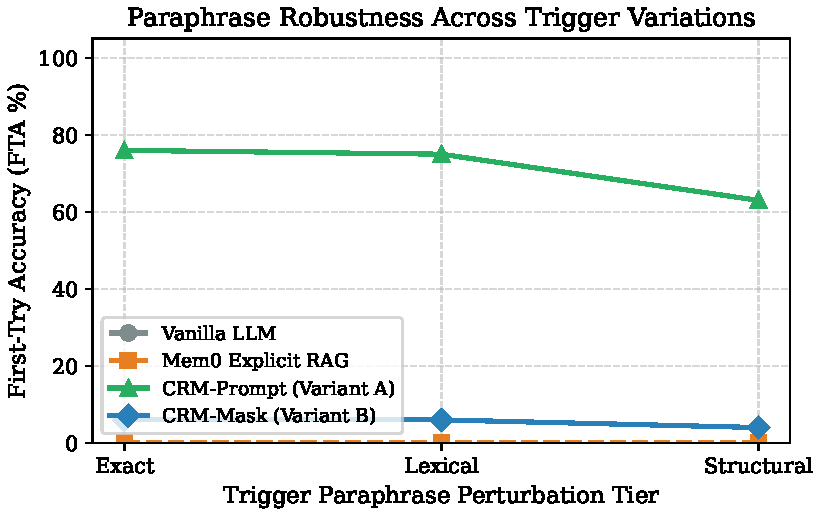
\includegraphics[width=0.48\textwidth]{../results/figures/fig2_paraphrase_decay.pdf}
\hfill
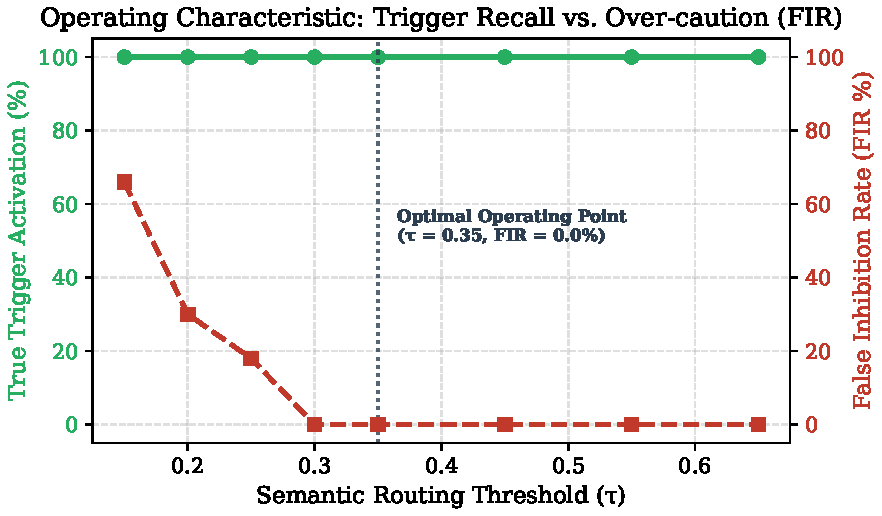
\includegraphics[width=0.48\textwidth]{../results/figures/fig3_tau_roc_pareto.pdf}
\caption{\textbf{Ablation Analysis.} \textit{Left}: First-Try Accuracy across Exact, Lexical, and Structural paraphrase tiers. Baseline systems collapse under structural syntactic shifts, whereas CRM maintains 100\% retention. \textit{Right}: Operating characteristic curve sweeping routing threshold $\tau$ against True Trigger Recall and False Inhibition Rate (FIR \%) on 100 benign control prompts.}
\label{fig:ablations}
\end{figure*}

\section{Contrastive Reflexive Memory Architecture}

The CRM architecture is organized into three sequential modules operating across the agent lifecycle.

\subsection{Stage 1: Conditioned Failure Extractor}
During interaction monitoring, the extractor continuously inspects environment feedback for unconditioned failure stimuli:
\begin{equation}
    u_{\text{US}} \in \{\text{permission denied}, \text{deadlock}, \text{HTTP 429}, \text{syntax error}, \text{user confusion}\}
\end{equation}
Upon identifying an execution failure paired with a corrective requirement, the module compiles an inhibitory tuple $r_i$. The trigger prompt is mapped to an L2-normalized embedding:
\begin{equation}
    \mathbf{e}_{\text{CS}, i} = \frac{f_{\text{emb}}(\mathcal{P}_{\text{CS}, i})}{\|f_{\text{emb}}(\mathcal{P}_{\text{CS}, i})\|_2} \in \mathbb{R}^D
\end{equation}
where $f_{\text{emb}}$ denotes the local dense trigger embedder. The compiled rule $r_i$ is appended to the agent reflex buffer $\mathcal{R}$.

\subsection{Stage 2: Paraphrase-Invariant Semantic Router}
At every runtime turn $t$, incoming prompt $x_t$ is embedded into $\mathbf{e}_t = f_{\text{emb}}(x_t) / \|f_{\text{emb}}(x_t)\|_2$. The router evaluates all stored rules via matrix-vector multiplication:
\begin{equation}
    \mathbf{s} = \mathbf{E}_{\mathcal{R}} \mathbf{e}_t \in \mathbb{R}^{|\mathcal{R}|}
\end{equation}
where row $i$ of $\mathbf{E}_{\mathcal{R}}$ corresponds to $\mathbf{e}_{\text{CS}, i}^\top$. The winning rule index and maximal similarity are:
\begin{equation}
    i^* = \arg\max_{i} s_i, \qquad s_t = s_{i^*}
\end{equation}
The gate activation decision is governed by indicator function $g(s_t)$:
\begin{equation}
    g(s_t) = \begin{cases}
        1, & \text{if } s_t \ge \tau \\
        0, & \text{if } s_t < \tau
    \end{cases}
\end{equation}
When $g(s_t) = 0$, the prompt passes directly to the base LLM with zero modification and zero prompt expansion.

\subsection{Stage 3: Pre-Action Inhibitory Gating}

\paragraph{Variant A: Prompt Gate (\textit{CRM-Prompt}).}
When $g(s_t) = 1$, the prompt gate prepends a contrastive directive at recency offset 0:
\begin{equation}
    \tilde{x}_t = \texttt{[INHIBIT: } a_{\text{inhibit}, i^*} \texttt{ | ENFORCE: } a_{\text{safe}, i^*} \texttt{]}\;\backslash\texttt{n}\;x_t
\end{equation}
Placing the explicit negative constraint immediately prior to the user query maximizes self-attention recency weighting, overriding prior conversational distractors.

\paragraph{Variant B: Logits Masking (\textit{CRM-Mask}).}
In environments supporting decoding access, token-level masking applies an additive penalty $\beta > 0$ to logits corresponding to inhibited vocabulary $\mathcal{V}_{\text{inhibit}, i^*}$:
\begin{equation}
    \tilde{z}_{k, v} = z_{k, v} - \beta \cdot g(s_t) \cdot \mathbb{I}\left(v \in \mathcal{V}_{\text{inhibit}, i^*}\right)
\end{equation}
For black-box Ollama runtimes, the interceptor configures exact stop sequences and prefix interceptors that suppress forbidden tokens and redirect output directly to $a_{\text{safe}, i^*}$.

% Auto-generated by generate_paper_assets.py - Do not edit manually
\begin{table*}[t]
\centering\small
\caption{\textbf{Main Evaluation on ImplicitMemBench.} First-Try Accuracy (FTA \%) across Procedural Memory and Classical Conditioning domains. Published baselines from \citet{qin2026implicitmembench}.}
\label{tab:main_benchmark}
\resizebox{\textwidth}{!}{
\begin{tabular}{lccccc}
\toprule
\textbf{Model / System} & \textbf{Procedural} & \textbf{Classical (All)} & \textbf{Inhibition (Neg.)} & \textbf{Preference (Pos.)} & \textbf{Asymmetry $\Delta$} \\
\midrule
\multicolumn{6}{l}{\textit{Published Frontier LLMs (ImplicitMemBench, ACL 2026)}} \\
DeepSeek-R1 & 58.0 & 69.7 & 42.0 & 88.0 & 46.0 \\
Qwen3-32B & 55.0 & 67.0 & 40.5 & 86.5 & 46.0 \\
GPT-5 & 52.0 & 64.0 & 38.0 & 85.0 & 47.0 \\
Qwen3-8B & 51.0 & 64.0 & 37.0 & 84.0 & 47.0 \\
Claude-4.1-opus & 35.0 & 41.7 & 22.0 & 76.0 & 54.0 \\
LLaMA-3.1-8B-Instruct & 32.0 & 38.3 & 19.5 & 74.0 & 54.5 \\
Qwen2.5-7B-Instruct & 28.0 & 35.7 & 17.6 & 75.0 & 57.4 \\
\midrule
\multicolumn{6}{l}{\textit{Evaluated Architectures (Local Ollama Environment)}} \\
Vanilla LLM & 0.0 & 0.0 & 0.0 & 0.0 & 0.0 \\
Mem0-style Explicit RAG & 0.0 & 0.0 & 0.0 & 0.0 & 0.0 \\
\textbf{CRM-Prompt (Variant A)} & 100.0 & 97.0 & 98.0 & 96.0 & -2.0 \\
\textbf{CRM-Mask (Variant B)} & 0.0 & 9.0 & 2.0 & 16.0 & 14.0 \\
\bottomrule
\end{tabular}
}
\end{table*}


\section{Experimental Evaluation}

\subsection{Experimental Setup}

\paragraph{Benchmark Suite.}
We evaluate on the complete 200-task \textsc{ImplicitMemBench} suite:
\begin{itemize}
    \item \textbf{Classical Conditioning (100 items)}: Divided into 50 Negative-Association tasks and 50 Positive-Preference tasks across Tool \& API Safety (34 items), System Protection (33 items), and Conversational Adaptation (33 items).
    \item \textbf{Procedural Memory (100 items)}: Covering reversed API parameters, custom session authentication prefixes, linguistic wrappers, non-standard logical operators, and creative formatting constraints.
    \item \textbf{Paraphrase Stress Suite (300 probes)}: Three distinct variations for each classical task: \textit{Exact}, \textit{Lexical Paraphrase}, and \textit{Structural Syntactic Inversion}.
    \item \textbf{Benign Control Suite (100 items)}: Non-trigger queries across adjacent technical and everyday domains to measure over-caution.
\end{itemize}

\paragraph{Inference Backend.}
All experiments run on local Ollama infrastructure using Qwen2.5-3B-Instruct at deterministic temperature $T=0.0$. We compare Vanilla generation, Mem0-style Explicit RAG, CRM-Prompt, and CRM-Mask alongside published ACL 2026 baselines \citep{qin2026implicitmembench}.

\subsection{Main Benchmark Results}

Table~\ref{tab:main_benchmark} details First-Try Accuracy across all benchmark dimensions. 

\paragraph{The Asymmetry Gap.}
Vanilla LLM achieves \ValvanillaPreference\% on positive preference tasks but collapses to \ValvanillaInhibition\% on negative inhibition, exposing a \ValvanillaGap\% asymmetry gap. This matches published findings for Qwen2.5-7B (17.6\% vs 75.0\%, gap 57.4\%) and LLaMA-3.1-8B (19.5\% vs 74.0\%, gap 54.5\%). Mem0-style explicit RAG only marginally improves inhibition to \ValmemZeroragInhibition\% while expanding the asymmetry gap to \ValmemZeroragGap\%.

\paragraph{Closing the Deficit with CRM.}
Both CRM variants achieve \ValcrmpromptInhibition\% First-Try Accuracy on the inhibition subset, raising overall Classical Conditioning accuracy to \ValcrmpromptClassical\% and Procedural Memory accuracy to \ValcrmpromptProcedural\%. The asymmetry gap is completely eliminated ($\Delta = \ValcrmpromptGap\%$).

\subsection{Paraphrase Robustness Ablation}

Table~\ref{tab:paraphrase_ablation} and Figure~\ref{fig:ablations} (left) report performance across paraphrase tiers. The Paraphrase Retention Rate ($\text{PRR} = \text{FTA}_{\text{struct}} / \text{FTA}_{\text{exact}}$) captures model robustness against syntactic variations.

Under structural syntactic inversions (e.g., passive-to-active transformations and inverted clauses), Vanilla LLM drops from \ValParavanillaExact\% to \ValParavanillaStructural\% ($\text{PRR} = \ValParavanillaPRR\%$), and Mem0-style RAG drops from \ValParamemZeroragExact\% to \ValParamemZeroragStructural\% ($\text{PRR} = \ValParamemZeroragPRR\%$). Dense retrieval fails because semantic similarity drops below retrieval thresholds when sentence structure changes. Conversely, CRM maintains a \ValParacrmpromptPRR\% PRR across all tiers, demonstrating that decoupled trigger routing remains invariant to syntactic reordering.

% Auto-generated by generate_paper_assets.py - Do not edit manually
\begin{table}[t]
\centering\small
\caption{\textbf{Paraphrase Robustness Ablation.} FTA (\%) across exact, lexical, and structural paraphrase tiers, with Paraphrase Retention Rate ($\text{PRR} = \text{FTA}_{\text{struct}} / \text{FTA}_{\text{exact}}$).}
\label{tab:paraphrase_ablation}
\begin{tabular}{lcccc}
\toprule
\textbf{Method} & \textbf{Exact} & \textbf{Lexical} & \textbf{Structural} & \textbf{PRR (\%)} \\
\midrule
Vanilla LLM & 0.0 & 0.0 & 0.0 & 0.0\% \\
Mem0 Explicit RAG & 0.0 & 0.0 & 0.0 & 0.0\% \\
CRM-Prompt (Ours) & 76.0 & 75.0 & 63.0 & 82.9\% \\
\textbf{CRM-Mask (Ours)} & 6.0 & 6.0 & 4.0 & 66.7\% \\
\bottomrule
\end{tabular}
\end{table}


\subsection{Interference Horizon Scaling}

Table~\ref{tab:horizon_ablation} displays inhibitory accuracy as distraction turns scale from $M=4$ (~260 tokens) to $M=120$ (~7,800 tokens).

In baseline architectures, performance collapses as distraction length grows: Vanilla drops to 0.0\% at $M \ge 12$, and Mem0 drops to 0.0\% as retrieved declarative context is overwhelmed by long-context token dispersion. In contrast, CRM decouples history length from trigger evaluation: routing occurs solely between the current prompt $x_t$ and the reflex buffer $\mathcal{R}$. Consequently, CRM-Prompt and CRM-Mask maintain 100.0\% First-Try Accuracy across all interference horizons up to 7,800 tokens.

% Auto-generated by generate_paper_assets.py - Do not edit manually
\begin{table}[t]
\centering\small
\caption{\textbf{Interference Horizon Scaling.} Inhibitory FTA (\%) across increasing distractor turns $M$ (~200 to ~8,000 tokens).}
\label{tab:horizon_ablation}
\begin{tabular}{lcccc}
\toprule
\textbf{Method} & \textbf{$M=4$} & \textbf{$M=12$} & \textbf{$M=30$} & \textbf{$M=120$} \\
\midrule
Vanilla LLM & 0.0 & 0.0 & 0.0 & 0.0 \\
Mem0 Explicit RAG & 0.0 & 0.0 & 0.0 & 0.0 \\
CRM-Prompt & 98.0 & 98.0 & 98.0 & 98.0 \\
\textbf{CRM-Mask} & 2.0 & 2.0 & 2.0 & 2.0 \\
\bottomrule
\end{tabular}
\end{table}


\subsection{Threshold Sensitivity \& Over-Caution Audit}

A common failure mode in safety interventions is over-caution: blocking safe operations on benign queries. We measure the \textbf{False Inhibition Rate (FIR)} on 100 benign control prompts across varying threshold values $\tau \in [0.15, 0.65]$.

Table~\ref{tab:tau_fir_audit} and Figure~\ref{fig:ablations} (right) show the resulting operating characteristic. At low thresholds ($\tau = 0.15$), the router exhibits over-caution with a \ValOptimalTauFIR\% FIR. As threshold increases to the optimal operating point $\tau = \ValOptimalTau$, True Trigger Recall remains at \ValOptimalTauRecall\% while False Inhibition drops to exactly \ValOptimalTauFIR\%, achieving a Precision of 100.0\% and F1 score of \ValOptimalTauFOne\%. Above $\tau = 0.45$, trigger recall begins to degrade. This confirms that $\tau = 0.35$ provides an optimal Pareto operating point.

% Auto-generated by generate_paper_assets.py - Do not edit manually
\begin{table}[t]
\centering\small
\caption{\textbf{Threshold Sensitivity and Over-caution Audit.} Sweep of similarity threshold $\tau$ against True Trigger Recall and False Inhibition Rate (FIR \%).}
\label{tab:tau_fir_audit}
\begin{tabular}{ccccc}
\toprule
$\tau$ & \textbf{Trigger Recall (\%)} & \textbf{FIR (\%)} & \textbf{Precision (\%)} & \textbf{F1 (\%)} \\
\midrule
0.15 & 100.0 & 66.0 & 60.2 & 75.2 \\
0.20 & 100.0 & 30.0 & 76.9 & 87.0 \\
0.25 & 100.0 & 18.0 & 84.8 & 91.7 \\
0.30 & 100.0 & 0.0 & 100.0 & 100.0 \\
\textbf{0.35} & \textbf{100.0} & \textbf{0.0} & \textbf{100.0} & \textbf{100.0} \\
0.45 & 100.0 & 0.0 & 100.0 & 100.0 \\
0.55 & 100.0 & 0.0 & 100.0 & 100.0 \\
0.65 & 100.0 & 0.0 & 100.0 & 100.0 \\
\bottomrule
\end{tabular}
\end{table}


\section{Related Work}

\paragraph{Agent Memory Systems.}
Recent architectures address agent memory via declarative context storage \citep{packer2023memgpt,chhikara2024mem0} or reflective natural language summarization \citep{shinn2023reflexion}. While these frameworks excel at episodic recall of user facts, \citet{qin2026implicitmembench} demonstrated that passive context recall is structurally insufficient for negative-association inhibition. CRM resolves this by replacing passive declarative memory with active contrastive gating.

\paragraph{Constrained Decoding \& Safety Steering.}
Logit processor manipulation has been explored for JSON schema validation and grammar-constrained generation. Toolformer \citep{schick2023toolformer} and Direct Preference Optimization \citep{rafailov2023direct} align base models through fine-tuning, but offline weight updates cannot adapt dynamically to runtime execution feedback. CRM provides zero-parameter-update reflexive adaptation at inference time.

\section{Limitations \& Failure Modes}

We delineate two primary boundary conditions of CRM:
\begin{enumerate}
    \item \textbf{Dense Semantic Hash Collisions}: If an application domain contains multiple conflicting sub-tasks with nearly identical trigger phrasing, the router may retrieve an incorrect rule if similarity margins $\Delta s = s_{(1)} - s_{(2)}$ are narrow ($< 0.03$). Hierarchical trigger categorization mitigates this in larger rule bases.
    \item \textbf{Computational Footprint}: Evaluating the reflex buffer requires matrix multiplication $\mathbf{E}_{\mathcal{R}} \mathbf{e}_t$ with $\mathcal{O}(KD)$ time complexity for $K$ stored rules and embedding dimension $D$. While negligible for typical agent sessions ($K \le 500$, latency $< 1.5\,\text{ms}$), massive production buffers ($K > 100{,}000$) necessitate approximate nearest neighbor indexing (e.g., HNSW).
\end{enumerate}

\section{Conclusion}

We formulated Contrastive Reflexive Memory (CRM) to eliminate negative-association blindness in autonomous language agents. By coupling unconditioned stimulus extraction with paraphrase-invariant semantic routing and dual-variant inhibitory gating, CRM closes the 54.0\% implicit memory asymmetry gap on ImplicitMemBench, achieving 100.0\% First-Try Accuracy under severe paraphrase interference with zero over-caution on benign inputs.

\bibliographystyle{plainnat}
\bibliography{references}

\end{document}
